\documentclass[11pt,a4paper,oneside]{report}             % Single-side
%\documentclass[11pt,a4paper,twoside,openright]{report}  % Duplex

% thanks to http://tex.stackexchange.com/a/47579/71109
\usepackage{ifxetex}
\usepackage{ifluatex}
\newif\ifxetexorluatex % a new conditional starts as false
\ifnum 0\ifxetex 1\fi\ifluatex 1\fi>0
   \xetexorluatextrue
\fi

\ifxetexorluatex
  \usepackage{fontspec}
\else
  \usepackage[T1]{fontenc}
  \usepackage[utf8]{inputenc}
  \usepackage[lighttt]{lmodern}
  \ttfamily\DeclareFontShape{T1}{lmtt}{m}{it}{<->sub*lmtt/m/sl}{}
\fi

\usepackage[english,magyar]{babel} % Alapértelmezés szerint utoljára definiált nyelv lesz aktív, de később külön beállítjuk az aktív nyelvet.

\usepackage{emptypage} % omit page number on empty pages

%\usepackage{cmap}
\usepackage{amsfonts,amsmath,amssymb} % Mathematical symbols.
%\usepackage[ruled,boxed,resetcount,linesnumbered]{algorithm2e} % For pseudocodes. % beware: this is not compatible with LuaLaTeX, see http://tex.stackexchange.com/questions/34814/lualatex-and-algorithm2e
\usepackage{booktabs} % For publication quality tables for LaTeX
\usepackage{graphicx}

%\usepackage{fancyhdr}
%\usepackage{lastpage}

\usepackage{geometry}
%\usepackage{sectsty}
\usepackage{setspace} % For setting line spacing

\usepackage[unicode]{hyperref} % For hyperlinks in the generated document.
\usepackage{xcolor}
\usepackage{listings} % For source code snippets.

\usepackage[amsmath,thmmarks]{ntheorem} % Theorem-like environments.

\usepackage[hang]{caption}

\singlespacing

\newcommand{\selecthungarian}{
	\selectlanguage{magyar}
	\setlength{\parindent}{2em}
	\setlength{\parskip}{0em}
	\frenchspacing
}

\newcommand{\selectenglish}{
	\selectlanguage{english}
	\setlength{\parindent}{0em}
	\setlength{\parskip}{0.5em}
	\nonfrenchspacing
	\renewcommand{\figureautorefname}{Figure}
	\renewcommand{\tableautorefname}{Table}
	\renewcommand{\partautorefname}{Part}
	\renewcommand{\chapterautorefname}{Chapter}
	\renewcommand{\sectionautorefname}{Section}
	\renewcommand{\subsectionautorefname}{Section}
	\renewcommand{\subsubsectionautorefname}{Section}
}

\usepackage[numbers]{natbib}
\usepackage{xspace}

\usepackage{minted}
%TODO Set the main variables
\newcommand{\vikszerzoVezeteknev}{Gilicze}
\newcommand{\vikszerzoKeresztnev}{Márton}

\newcommand{\vikkonzulensAMegszolitas}{}
\newcommand{\vikkonzulensAVezeteknev}{Szántó}
\newcommand{\vikkonzulensAKeresztnev}{Péter}

%\newcommand{\vikkonzulensBMegszolitas}{}
%\newcommand{\vikkonzulensBVezeteknev}{Konzulens}
%\newcommand{\vikkonzulensBKeresztnev}{Kettő}

%\newcommand{\vikkonzulensCMegszolitas}{}
%\newcommand{\vikkonzulensCVezeteknev}{}
%\newcommand{\vikkonzulensCKeresztnev}{}

\newcommand{\vikcim}{Videó átméretező megvalósítása FPGA-val} % Cím
\newcommand{\viktanszek}{\bmemit} % Tanszék
\newcommand{\vikdoktipus}{\msc} % Dokumentum típusa (\bsc vagy \msc)
\newcommand{\vikmunkatipusat}{Önálló laboratórium 1} % a "hallgató nyilatkozat" részhez: szakdolgozatot vagy diplomatervet

%--------------------------------------------------------------------------------------
% TDK-specifikus változók
%--------------------------------------------------------------------------------------
\newcommand{\tdkszerzoB}{Második Szerző} % Második szerző neve; hagyd üresen, ha egyedül írtad a TDK-t.
\newcommand{\tdkev}{2014} % A dolgozat írásának éve (pl. "2014") (Ez OTDK-nál eltérhet az aktuális évtől.)

% További adatok az OTDK címlaphoz (BME-s TDK-hoz nem kell kitölteni)
\newcommand{\tdkevfolyamA}{IV} % Első szerző évfolyama, római számmal (pl. IV).
\newcommand{\tdkevfolyamB}{III} % Második szerző évfolyama, római számmal (pl. III).
\newcommand{\tdkkonzulensbeosztasA}{egyetemi tanár} % Első konzulens beosztása (pl. egyetemi docens)
\newcommand{\tdkkonzulensbeosztasB}{doktorandusz} % Második konzulens beosztása (pl. egyetemi docens)

\newcommand{\szerzoMeta}{\vikszerzoVezeteknev{} \vikszerzoKeresztnev} % egy szerző esetén
%\newcommand{\szerzoMeta}{\vikszerzoVezeteknev{} \vikszerzoKeresztnev, \tdkszerzoB} % két szerző esetén

%TODO Language configuration -- choose one
% Beállítások magyar nyelvű dolgozathoz
%--------------------------------------------------------------------------------------
% Elnevezések
%--------------------------------------------------------------------------------------
\newcommand{\bme}{Budapesti Műszaki és Gazdaságtudományi Egyetem}
\newcommand{\vik}{Villamosmérnöki és Informatikai Kar}

\newcommand{\bmemit}{Méréstechnika és Információs Rendszerek Tanszék}

\newcommand{\keszitette}{Készítette}
\newcommand{\konzulens}{Konzulens}

\newcommand{\bsc}{Szakdolgozat}
\newcommand{\msc}{Diplomaterv}
\newcommand{\tdk}{TDK dolgozat}
\newcommand{\bsconlab}{BSc Önálló laboratórium}
\newcommand{\msconlabi}{MSc Önálló laboratórium 1.}
\newcommand{\msconlabii}{MSc Önálló laboratórium 2.}

\newcommand{\pelda}{Példa}
\newcommand{\definicio}{Definíció}
\newcommand{\tetel}{Tétel}

\newcommand{\bevezetes}{Bevezetés}
\newcommand{\koszonetnyilvanitas}{Köszönetnyilvánítás}
\newcommand{\fuggelek}{Függelék}

% Opcionálisan átnevezhető címek
%\addto\captionsmagyar{%
%\renewcommand{\listfigurename}{Saját ábrajegyzék cím}
%\renewcommand{\listtablename}{Saját táblázatjegyzék cím}
%\renewcommand{\bibname}{Saját irodalomjegyzék név}
%}

\newcommand{\szerzo}{\vikszerzoVezeteknev{} \vikszerzoKeresztnev}
\newcommand{\vikkonzulensA}{\vikkonzulensAMegszolitas\vikkonzulensAVezeteknev{} \vikkonzulensAKeresztnev}
\newcommand{\vikkonzulensB}{\vikkonzulensBMegszolitas\vikkonzulensBVezeteknev{} \vikkonzulensBKeresztnev}
\newcommand{\vikkonzulensC}{\vikkonzulensCMegszolitas\vikkonzulensCVezeteknev{} \vikkonzulensCKeresztnev}

\newcommand{\selectthesislanguage}{\selecthungarian}

\bibliographystyle{huplain}

\def\lstlistingname{lista}

\newcommand{\appendixnumber}{6}  % a fofejezet-szamlalo az angol ABC 6. betuje (F) lesz

% Settings for English documents
%%--------------------------------------------------------------------------------------
% Elnevezések
%--------------------------------------------------------------------------------------
\newcommand{\bme}{Budapest University of Technology and Economics}
\newcommand{\vik}{Faculty of Electrical Engineering and Informatics}

\newcommand{\bmemit}{Department of Measurement and Information Systems}

\newcommand{\keszitette}{Author}
\newcommand{\konzulens}{Advisor}

\newcommand{\bsc}{Bachelor's Thesis}
\newcommand{\msc}{Master's Thesis}
\newcommand{\tdk}{Scientific Students' Association Report}
\newcommand{\bsconlab}{BSc Project Laboratory}
\newcommand{\msconlabi}{MSc Project Laboratory 1}
\newcommand{\msconlabii}{MSc Project Laboratory 2}

\newcommand{\pelda}{Example}
\newcommand{\definicio}{Definition}
\newcommand{\tetel}{Theorem}

\newcommand{\bevezetes}{Introduction}
\newcommand{\koszonetnyilvanitas}{Acknowledgements}
\newcommand{\fuggelek}{Appendix}

% Optional custom titles
%\addto\captionsenglish{%
%\renewcommand*{\listfigurename}{Your list of figures title}
%\renewcommand*{\listtablename}{Your list of tables title}
%\renewcommand*{\bibname}{Your bibliography title}
%}

\newcommand{\szerzo}{\vikszerzoKeresztnev{} \vikszerzoVezeteknev}
\newcommand{\vikkonzulensA}{\vikkonzulensAMegszolitas\vikkonzulensAKeresztnev{} \vikkonzulensAVezeteknev}
\newcommand{\vikkonzulensB}{\vikkonzulensBMegszolitas\vikkonzulensBKeresztnev{} \vikkonzulensBVezeteknev}
\newcommand{\vikkonzulensC}{\vikkonzulensCMegszolitas\vikkonzulensCKeresztnev{} \vikkonzulensCVezeteknev}

\newcommand{\selectthesislanguage}{\selectenglish}

\bibliographystyle{plainnat}

\newcommand{\ie}{i.e.\@\xspace}
\newcommand{\Ie}{I.e.\@\xspace}
\newcommand{\eg}{e.g.\@\xspace}
\newcommand{\Eg}{E.g.\@\xspace}
\newcommand{\etal}{et al.\@\xspace}
\newcommand{\etc}{etc.\@\xspace}
\newcommand{\vs}{vs.\@\xspace}
\newcommand{\viz}{viz.\@\xspace} % videlicet
\newcommand{\cf}{cf.\@\xspace} % confer
\newcommand{\Cf}{Cf.\@\xspace}
\newcommand{\wrt}{w.r.t.\@\xspace} % with respect to
\newcommand{\approximately}{approx.\@\xspace}

\newcommand{\appendixnumber}{1}  % a fofejezet-szamlalo az angol ABC 1. betuje (A) lesz


%--------------------------------------------------------------------------------------
% Page layout setup
%--------------------------------------------------------------------------------------
% we need to redefine the pagestyle plain
% another possibility is to use the body of this command without \fancypagestyle
% and use \pagestyle{fancy} but in that case the special pages
% (like the ToC, the References, and the Chapter pages)remain in plane style

\pagestyle{plain}
\geometry{inner=35mm, outer=25mm, top=28mm, bottom=25mm}

\setcounter{tocdepth}{3}
%\sectionfont{\large\upshape\bfseries}
\setcounter{secnumdepth}{3}

\sloppy % Margón túllógó sorok tiltása.
\widowpenalty=10000 \clubpenalty=10000 %A fattyú- és árvasorok elkerülése
\def\hyph{-\penalty0\hskip0pt\relax} % Kötőjeles szavak elválasztásának engedélyezése


%--------------------------------------------------------------------------------------
% Setup hyperref package
%--------------------------------------------------------------------------------------
\hypersetup{
    % bookmarks=true,            % show bookmarks bar?
    unicode=true,              % non-Latin characters in Acrobat's bookmarks
    pdftitle={\vikcim},        % title
    pdfauthor={\szerzoMeta},    % author
    pdfsubject={\vikdoktipus}, % subject of the document
    pdfcreator={\szerzoMeta},   % creator of the document
    pdfproducer={},    % producer of the document
    pdfkeywords={},    % list of keywords (separate then by comma)
    pdfnewwindow=true,         % links in new window
    colorlinks=true,           % false: boxed links; true: colored links
    linkcolor=black,           % color of internal links
    citecolor=black,           % color of links to bibliography
    filecolor=black,           % color of file links
    urlcolor=black             % color of external links
}


%--------------------------------------------------------------------------------------
% Set up listings
%--------------------------------------------------------------------------------------
\definecolor{lightgray}{rgb}{0.95,0.95,0.95}
\lstset{
	basicstyle=\scriptsize\ttfamily, % print whole listing small
	keywordstyle=\color{black}\bfseries, % bold black keywords
	identifierstyle=, % nothing happens
	% default behavior: comments in italic, to change use
	% commentstyle=\color{green}, % for e.g. green comments
	stringstyle=\scriptsize,
	showstringspaces=false, % no special string spaces
	aboveskip=3pt,
	belowskip=3pt,
	backgroundcolor=\color{lightgray},
	columns=flexible,
	keepspaces=true,
	escapeinside={(*@}{@*)},
	captionpos=b,
	breaklines=true,
	frame=single,
	float=!ht,
	tabsize=2,
	literate=*
		{á}{{\'a}}1	{é}{{\'e}}1	{í}{{\'i}}1	{ó}{{\'o}}1	{ö}{{\"o}}1	{ő}{{\H{o}}}1	{ú}{{\'u}}1	{ü}{{\"u}}1	{ű}{{\H{u}}}1
		{Á}{{\'A}}1	{É}{{\'E}}1	{Í}{{\'I}}1	{Ó}{{\'O}}1	{Ö}{{\"O}}1	{Ő}{{\H{O}}}1	{Ú}{{\'U}}1	{Ü}{{\"U}}1	{Ű}{{\H{U}}}1
}


%--------------------------------------------------------------------------------------
% Set up theorem-like environments
%--------------------------------------------------------------------------------------
% Using ntheorem package -- see http://www.math.washington.edu/tex-archive/macros/latex/contrib/ntheorem/ntheorem.pdf

\theoremstyle{plain}
\theoremseparator{.}
\newtheorem{example}{\pelda}

\theoremseparator{.}
%\theoremprework{\bigskip\hrule\medskip}
%\theorempostwork{\hrule\bigskip}
\theorembodyfont{\upshape}
\theoremsymbol{{\large \ensuremath{\centerdot}}}
\newtheorem{definition}{\definicio}

\theoremseparator{.}
%\theoremprework{\bigskip\hrule\medskip}
%\theorempostwork{\hrule\bigskip}
\newtheorem{theorem}{\tetel}


%--------------------------------------------------------------------------------------
% Some new commands and declarations
%--------------------------------------------------------------------------------------
\newcommand{\code}[1]{{\upshape\ttfamily\scriptsize\indent #1}}
\newcommand{\doi}[1]{DOI: \href{http://dx.doi.org/\detokenize{#1}}{\raggedright{\texttt{\detokenize{#1}}}}} % A hivatkozások közt így könnyebb DOI-t megadni.

\DeclareMathOperator*{\argmax}{arg\,max}
%\DeclareMathOperator*[1]{\floor}{arg\,max}
\DeclareMathOperator{\sign}{sgn}
\DeclareMathOperator{\rot}{rot}


%--------------------------------------------------------------------------------------
% Setup captions
%--------------------------------------------------------------------------------------
\captionsetup[figure]{aboveskip=10pt}

\renewcommand{\captionlabelfont}{\bf}
%\renewcommand{\captionfont}{\footnotesize\it}

%--------------------------------------------------------------------------------------
% Hyphenation exceptions
%--------------------------------------------------------------------------------------
\hyphenation{Shakes-peare Mar-seilles ár-víz-tű-rő tü-kör-fú-ró-gép}


\author{\vikszerzo}
\title{\viktitle}


%--------------------------------------------------------------------------------------
% Table of contents and the main text
%--------------------------------------------------------------------------------------
\begin{document}

\pagenumbering{gobble}

%TODO These includes define guidelines -- remove these
%~~~~~~~~~~~~~~~~~~~~~~~~~~~~~~~~~~~~~~~~~~~~~~~~~~~~~~~~~~~~~~~~~~~~~~~~~~~~~~~~~~~~~~
%\selecthungarian
%--------------------------------------------------------------------------------------
% Rovid formai es tartalmi tajekoztato
%--------------------------------------------------------------------------------------

\footnotesize
\begin{center}
\large
\textbf{\Large Általános információk, a diplomaterv szerkezete}\\
\end{center}

A diplomaterv szerkezete a BME Villamosmérnöki és Informatikai Karán:
\begin{enumerate}
\item	Diplomaterv feladatkiírás
\item	Címoldal
\item	Tartalomjegyzék
\item	A diplomatervező nyilatkozata az önálló munkáról és az elektronikus adatok kezeléséről
\item	Tartalmi összefoglaló magyarul és angolul
\item	Bevezetés: a feladat értelmezése, a tervezés célja, a feladat indokoltsága, a diplomaterv felépítésének rövid összefoglalása
\item	A feladatkiírás pontosítása és részletes elemzése
\item	Előzmények (irodalomkutatás, hasonló alkotások), az ezekből levonható következtetések
\item	A tervezés részletes leírása, a döntési lehetőségek értékelése és a választott megoldások indoklása
\item	A megtervezett műszaki alkotás értékelése, kritikai elemzése, továbbfejlesztési lehetőségek
\item	Esetleges köszönetnyilvánítások
\item	Részletes és pontos irodalomjegyzék
\item	Függelék(ek)
\end{enumerate}

Felhasználható a következő oldaltól kezdődő \LaTeX diplomatervsablon dokumentum tartalma. 

A diplomaterv szabványos méretű A4-es lapokra kerüljön. Az oldalak tükörmargóval készüljenek (mindenhol 2,5~cm, baloldalon 1~cm-es kötéssel). Az alapértelmezett betűkészlet a 12 pontos Times New Roman, másfeles sorközzel, de ettől kismértékben el lehet térni, ill. más betűtípus használata is megengedett.

Minden oldalon -- az első négy szerkezeti elem kivételével -- szerepelnie kell az oldalszámnak.

A fejezeteket decimális beosztással kell ellátni. Az ábrákat a megfelelő helyre be kell illeszteni, fejezetenként decimális számmal és kifejező címmel kell ellátni. A fejezeteket decimális aláosztással számozzuk, maximálisan 3 aláosztás mélységben (pl. 2.3.4.1.). Az ábrákat, táblázatokat és képleteket célszerű fejezetenként külön számozni (pl. 2.4. ábra, 4.2. táblázat vagy képletnél (3.2)). A fejezetcímeket igazítsuk balra, a normál szövegnél viszont használjunk sorkiegyenlítést. Az ábrákat, táblázatokat és a hozzájuk tartozó címet igazítsuk középre. A cím a jelölt rész alatt helyezkedjen el.

A képeket lehetőleg rajzoló programmal készítsék el, az egyenleteket egyenlet-szerkesztő segítségével írják le (A \LaTeX~ehhez kézenfekvő megoldásokat nyújt).

Az irodalomjegyzék szövegközi hivatkozása történhet sorszámozva (ez a preferált megoldás) vagy a Harvard-rendszerben (a szerző és az évszám megadásával). A teljes lista névsor szerinti sorrendben a szöveg végén szerepeljen (sorszámozott irodalmi hivatkozások esetén hivatkozási sorrendben). A szakirodalmi források címeit azonban mindig az eredeti nyelven kell megadni, esetleg zárójelben a fordítással. A listában szereplő valamennyi publikációra hivatkozni kell a szövegben (a \LaTeX-sablon a Bib\TeX~segítségével mindezt automatikusan kezeli). Minden publikáció a szerzők után a következő adatok szerepelnek: folyóirat cikkeknél a pontos cím, a folyóirat címe, évfolyam, szám, oldalszám tól-ig. A folyóiratok címét csak akkor rövidítsük, ha azok nagyon közismertek vagy nagyon hosszúak. Internetes hivatkozások megadásakor fontos, hogy az elérési út előtt megadjuk az oldal tulajdonosát és tartalmát (mivel a link egy idő után akár elérhetetlenné is válhat), valamint az elérés időpontját.

\vspace{5mm}
Fontos:
\begin{itemize}
	\item A szakdolgozatkészítő / diplomatervező nyilatkozata (a jelen sablonban szereplő szövegtartalommal) kötelező előírás, Karunkon ennek hiányában a szakdolgozat/diplomaterv nem bírálható és nem védhető!
	\item Mind a dolgozat, mind a melléklet maximálisan 15~MB méretű lehet!
\end{itemize}

\vspace{5mm}
\begin{center}
Jó munkát, sikeres szakdolgozatkészítést, ill. diplomatervezést kívánunk!
\end{center}

\normalsize
\selectthesislanguage

%%--------------------------------------------------------------------------------------
% Feladatkiiras (a tanszeken atveheto, kinyomtatott valtozat)
%--------------------------------------------------------------------------------------
\clearpage
\begin{center}
\large
\textbf{FELADATKIÍRÁS}\\
\end{center}

A feladatkiírást a tanszéki adminisztrációban lehet átvenni, és a leadott munkába eredeti, tanszéki pecséttel ellátott és a tanszékvezető által aláírt lapot kell belefűzni (ezen oldal \emph{helyett}, ez az oldal csak útmutatás). Az elektronikusan feltöltött dolgozatban már nem kell beleszerkeszteni ezt a feladatkiírást.


\selectthesislanguage

%TODO Titlepage -- choose one from below
%~~~~~~~~~~~~~~~~~~~~~~~~~~~~~~~~~~~~~~~~~~~~~~~~~~~~~~~~~~~~~~~~~~~~~~~~~~~~~~~~~~~~~~
\hypersetup{pageanchor=false}
%--------------------------------------------------------------------------------------
%	The title page
%--------------------------------------------------------------------------------------
\begin{titlepage}
\begin{center}

\includegraphics[width=60mm,keepaspectratio]{figures/bme_logo.pdf}\\
\vspace{0.3cm}
\textbf{\bme}\\
\textmd{\vik}\\
\textmd{\viktanszek}\\[5cm]

\vspace{0.4cm}
{\huge \bfseries \vikcim}\\[0.8cm]
\vspace{0.5cm}
\textsc{\Large Önálló laboratórium 1}\\[4cm]

{
	\renewcommand{\arraystretch}{0.85}
	\begin{tabular}{cc}
	 \makebox[7cm]{\emph{\keszitette}} & \makebox[7cm]{\emph{\konzulens}} \\ \noalign{\smallskip}
	 \makebox[7cm]{\szerzo} & \makebox[7cm]{\vikkonzulensA} \\
	\end{tabular}
}

\vfill
{\large \today}
\end{center}
\end{titlepage}
\hypersetup{pageanchor=false}

		   % Szakdolgozat/Diplomaterv címlap
%%% TDK címlap
\begin{titlepage}
  \begin{center}  
  
\includegraphics[width=7cm]{./figures/bme_logo.pdf}
  \vspace{0.3cm}
  
  \bme \\
  \vik \\
  \viktanszek \\
  \vspace{5cm}
  
  \huge {\vikcim}
  \vspace{1.5cm}
  
  \large {\textbf{\tdk}}
  \vfill
    
  {\Large 
  	\keszitette: \\ \vspace{0.3cm}
  	\szerzo \\
	\tdkszerzoB \\
  	\vspace{1.5cm}
  	\konzulens: \\ \vspace{0.3cm}
  	\vikkonzulensA \\
  	\vikkonzulensB \\
  }
  
  \vspace{2cm}
  \large {\tdkev}
 \end{center}
\end{titlepage}
%% Címlap vége
	% TDK címlap
%%% OTDK külső címlap
\begin{titlepage}
  	$\;$ 
	\vspace{5cm}
	
	\begin{center}
	\Huge
	\textbf{TDK-dolgozat}\let\thefootnote\relax\footnote{A dolgozat bemutatását a XXXXXXXXX  ``Lorem ipsum dolor sit amet'' című program támogatta.}
	\end{center}
	
	\vspace{13cm}
	
	\Large
	\hspace{8cm} \szerzo
	
	\hspace{8cm} \tdkszerzoB
	
	\hspace{8cm} \tdkev.
\end{titlepage}

\newpage
\thispagestyle{empty}


%% OTDK belső címlap
\begin{titlepage}
  \begin{center}  
  
\includegraphics[width=7cm]{./figures/bme_logo.pdf}
  \vspace{0.3cm}
  
  \bme \\
  \vik \\
  \viktanszek \\
  \vspace{3.5cm}
  
  \huge {\vikcim}
  \vspace{1.5cm}
  
  \large {\textbf{\vikdoktipus}}
  \vfill
    
  {\Large 
  	{\large \keszitette:} \\ \vspace{0.2cm}
  	\szerzo \\ \tdkevfolyamA. évfolyam \\
	\vspace{0.5cm}
	\tdkszerzoB \\ \tdkevfolyamB. évfolyam \\
  	\vspace{1.5cm}
  	{\large \konzulens:} \\ \vspace{0.2cm}
  	\vikkonzulensA,\\ \tdkkonzulensbeosztasA \\
  	\vspace{0.5cm}
  	\vikkonzulensB,\\ \tdkkonzulensbeosztasB \\
  }
  
  \vspace{2cm}
  \large {\tdkev.}
  
 \end{center}
\end{titlepage}   % OTDK címlap


% Declaration and Abstract
%~~~~~~~~~~~~~~~~~~~~~~~~~~~~~~~~~~~~~~~~~~~~~~~~~~~~~~~~~~~~~~~~~~~~~~~~~~~~~~~~~~~~~~
%\selectlanguage{magyar}
\pagenumbering{gobble}
%--------------------------------------------------------------------------------------
% Nyilatkozat
%--------------------------------------------------------------------------------------
\begin{center}
\large
\textbf{HALLGATÓI NYILATKOZAT}\\
\end{center}

Alulírott \emph{\vikszerzoVezeteknev{} \vikszerzoKeresztnev}, szigorló hallgató kijelentem, hogy ezt a \vikmunkatipusat{} meg nem engedett segítség nélkül, saját magam készítettem, csak a megadott forrásokat (szakirodalom, eszközök stb.) használtam fel. Minden olyan részt, melyet szó szerint, vagy azonos értelemben, de átfogalmazva más forrásból átvettem, egyértelműen, a forrás megadásával megjelöltem.

Hozzájárulok, hogy a jelen munkám alapadatait (szerző(k), cím, angol és magyar nyelvű tartalmi kivonat, készítés éve, konzulens(ek) neve) a BME VIK nyilvánosan hozzáférhető elektronikus formában, a munka teljes szövegét pedig az egyetem belső hálózatán keresztül (vagy autentikált felhasználók számára) közzétegye. Kijelentem, hogy a benyújtott munka és annak elektronikus verziója megegyezik. Dékáni engedéllyel titkosított diplomatervek esetén a dolgozat szövege csak 3 év eltelte után válik hozzáférhetővé.

\begin{flushleft}
\vspace*{1cm}
Budapest, \today
\end{flushleft}

\begin{flushright}
 \vspace*{1cm}
 \makebox[7cm]{\rule{6cm}{.4pt}}\\
 \makebox[7cm]{\emph{\vikszerzoVezeteknev{} \vikszerzoKeresztnev}}\\
 \makebox[7cm]{hallgató}
\end{flushright}
\thispagestyle{empty}

\vfill
\cleardoublepage

\selectthesislanguage
 %TODO Hallgatói nyilatkozat -- TDK és OTDK esetén törlendő!
\pagenumbering{roman}
\setcounter{page}{1}

\selecthungarian

%----------------------------------------------------------------------------
% Abstract in Hungarian
%----------------------------------------------------------------------------
\chapter*{Feladatkiírás}\addcontentsline{toc}{chapter}{Kivonat}

Az átméretezés igénye számos videó feldolgozó folyamatban merül fel igényként, s mivel a videó feldolgozás FPGA-ban tipikusan jól  megvalósítható feladat, így ebben a környezetben is szükség van az ezt a feladatot ellátó egységre.

Ugyan mindkét nagy FPGA gyártó (Intel, Xilinx) rendelkezik ehhez gyári megoldással, azonban ezek az IP magok meglehetősen drágák, és utóbbi gyártó esetén ráadásul meglehetősen rosszul működik. A feladat célja egy saját, általánosan használható átméretező IP kifejlesztése.

A cél egy olyan blokk kifejlesztése, amely testzőleges felbontásról képes bármilyen másik tetszőleges felbontásra skálázni magasabb fokszámű szűrők használatával, azaz jó minőségben.



\vfill
\cleardoublepage

\selectthesislanguage

\newcounter{romanPage}
\setcounter{romanPage}{\value{page}}
\stepcounter{romanPage}    %TODO Összefoglaló -- TDK és OTDK esetén nem kötelező

% Table of Contents
%~~~~~~~~~~~~~~~~~~~~~~~~~~~~~~~~~~~~~~~~~~~~~~~~~~~~~~~~~~~~~~~~~~~~~~~~~~~~~~~~~~~~~~
\tableofcontents\cleardoublepage


% The main part of the thesis
%~~~~~~~~~~~~~~~~~~~~~~~~~~~~~~~~~~~~~~~~~~~~~~~~~~~~~~~~~~~~~~~~~~~~~~~~~~~~~~~~~~~~~~
\pagenumbering{arabic}

%TODO import your own content
%----------------------------------------------------------------------------
\chapter{\bevezetes}
%----------------------------------------------------------------------------

A feladat során egy olyan videó átméretező IP blokk fejlesztését kezdtem meg, amely tetszőleges méretről tetszőleges méretre tud átméretezni videófolyamot. A videó átméretezésnek több alkalmazása is lehet, pl retro konzolok képeinek upscalelése nagyobb felbontásra, de egy érdekesebb felhasználása az a mesterséges intelligenciára épülő képfeldolgozásban van, ugyanis sok ilyen modell csak bizonyos méretű képeket/videókat képes bemenetként elfogadni, és ha pl a kameránk nem ilyen videófolyamot készít, akkor az mindenképpen preprocessingre szorul.

Azért választottam ezt a feladatot, hogy jobban megismerkedjek az FPGA-kal, és a digitális tervezéssel, hiszen eddigi tanulmányaim során nem találkoztam még velük. Éppen ezért a félév első felében főleg ismerkedtem a verilog nyelvvel, és a digitális tervezéssel, közben irodalomkutatást végeztem. A félév második felében pedig elkezdtem az implementációt.

A félév során azt a célt tűztem ki, hogy képeket legyen képes a modul tetszőleges méretűre átméretezni. Azzal, hogy a bemenő képfolyam milyen módon érkezik meg az FPGA-ba, jelenleg nem foglalkoztam.

Első lépének irodalomkutatást végeztem képek átméretezéséről. Itt különböző átméretezési algoritmusokat ismertem meg, melyek közül a bilineáris transzformációval, és a polyphase transzformációval foglalkoztam részletesebben.
 
Második lépésnek megpróbáltam egy egyszerűbb bilineáris algoritmust megvalósítani, amely tetszőleges méretről tetszőleges méretűre tud képeket átméretezni.

Harmadik lépésnek létrehoztam egy sorbuffer modult testbenchel, amely a megfelelő sorokat képes eltárolni egy bejövő folyamból, és a megfelelő pixeleket tudja adagolni az átméretező algoritmusnak.

Végezetül ezeket integráltam és test benchet hoztam létre nekik.
%----------------------------------------------------------------------------
\chapter{Irodalomkutatás}
\label{sec:LatexTools}
%----------------------------------------------------------------------------
\section{Létező megoldások keresése}
%----------------------------------------------------------------------------

Első lépésnek megpróbáltam már létező videó átméretező IP-ket keresni az interneten. Az Intel\cite{intelscaler}-nek és Xilinx\cite{xilinxscaler}-nek vannak már meglévő megoldásai, azonban ezek nem működnek mindig, sokszor hibásak, és van amit már nem is támogatnak. A két nagy gyártó saját scaler-jén kívül találtam harmadik féltől való megoldást is\cite{zipcores}, de ez is meglehetősen drága, úgyhogy egy saját IP kifejlesztésének igenis létjogosultsága van.

\section{Kép átméretezés}

Első lépésnek irodalomkutatást végeztem a képátméretezési technikákról. A képátméretezési technikák 2 fő csoportba oszthatóak: forward mapping és backward mapping.

\subsection{Forward mapping}

A forward mapping során egy bemeneti képnek a pixeleit próbáljuk közvetlenül átmappolni a kimeneti képnek a pixeleire. Ezt a \ref{pic:mapping} ábrán láthatjuk.  A kimeneti képen a képpontok ilyenkor nem fognak minden esetben pontosan ráesni egy-egy pixelre, ami miatt lyukak keletkezhetnek a kimeneti kép pixelei között. Erre egy lehetséges megoldás az, hogy az eredeti lép pixeleinek éleit vesszük, és ezt a formát átalakítjuk a kimeneti képre, majd ezután egy pixel értékét annak alapján állítjuk be, hogy az eredeti pixel értéke milyen mértékben van jelen ott. \cite{forwardmapping}

Ezek miatt belátható, hogy nem olyan szerencsés ezt a stratégiát használni. Sokkal jobb lenne, ha a kimeneti kép pixeleit mappolnánk át a bemeneti kép pixeleire, hiszen így biztosan minden kimeneti pixelre esne valamilyen érték. Ezt hívjuk backwards mappingnak.

\subsection{Backward mapping}

A backward mapping során fordítva, a kimeneti kép pixeleit feleltetjük meg a bemeneti kép pixeleihez. Ekkor ugyan szintén fenn áll a forward mapping során levő probléma, miszerint a pixelek nem fognak egy-egy pixelre ráesni a bemeneti képen, de ez itt nem probléma, hiszen itt minden pixel értékét ismerjük, tehát approximálhatjuk a nem egész koordinátán levő pixel értékét valamilyen algoritmus szerint. A \ref{pic:mapping} ábrán egy összehasonlítás látható a backward és forward mapping működése között.

\begin{figure}[!ht]
	\centering
	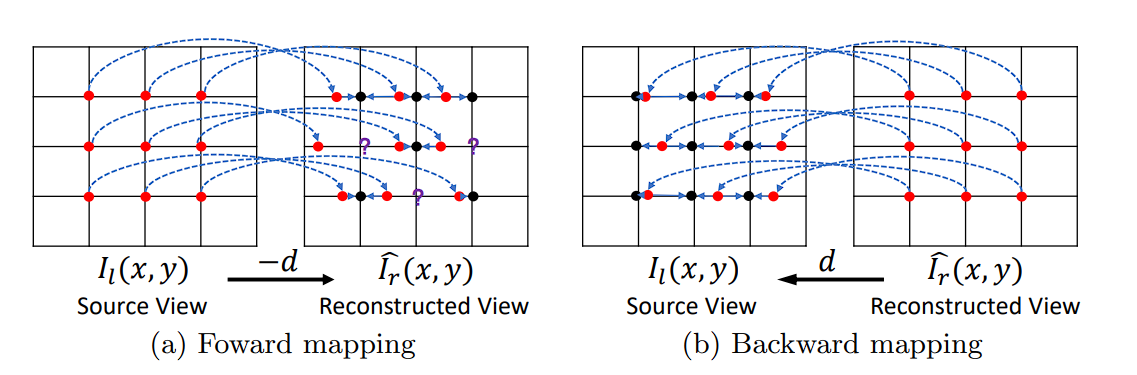
\includegraphics[width=120mm, keepaspectratio]{figures/mapping.png}
	\caption{A backward és forward mapping összehasonlítása \cite{forwardbackward}} 
	\label{pic:mapping}
\end{figure}

A projekt során a backward mapping megoldást használtam, hiszen ennek felhasználásával, könnyen lehet a kimeneti kép pixeleit a bemeneti képen való elhelyezkedésük alapján valamilyen algoritmus segítségével  meghatározni. Most tekintsünk meg néhány ilyen átméretező algoritmust.

\section{Bilinear filter}

A bilineáris szűrő az egyik egyszerűbb átméretezési technika. A lényege az, hogy a backward mapping során egy kimeneti pixelnek meghatározzuk a koordinátáját a bemeneti képen. Ez vagy ráesik egy pixelre, vagy nem. Ha nem esik rá egy pixelre teljesen, akkor viszont approximálni lehet az értékét a környező 4 pixel értékéből. A bilineáris interpoláció, mint a neve is mondja, 2 lineáris interpolációt végez el, vízszintesen, meg függőlegesen. A súlyok ilyenkor a környező pixelektől levő távolságok lesznek. Tehát egy 1D-s esetet nézve, ha a bal oldali pixelhez 2-szer olyan közel van a pixel mint a jobb oldalihoz, akkor a súlyok 0.66 és 0.33 lesznek. \cite{Wikipediabilinear_2024} A \ref{pic:bilinear} ábrán látható a vizualizációja az interpolációknak.

\begin{figure}[!ht]
	\centering
	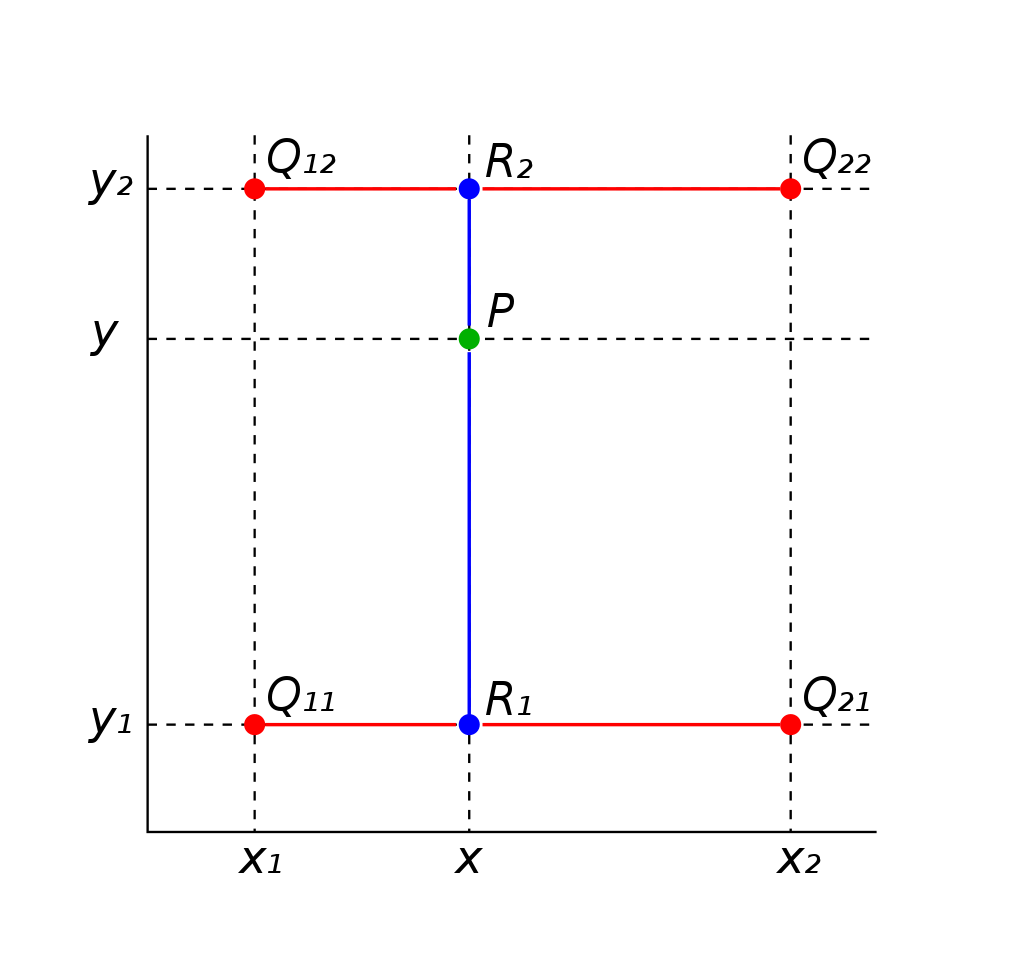
\includegraphics[width=100mm, keepaspectratio]{figures/bilinear.png}
	\caption{A bilineáris filter működése \cite{Wikipediabilinear_2024}} 
	\label{pic:bilinear}
\end{figure}
\newpage

A gyakorlatban 3 interpolációt kell megvalósítani, amiből a vízszintes irányban levő 2 interpolációt egyszerre, és utána pedig a függőleges interpolációt lehet elvégezni, ami már a kimenete lesz a filternek. A legegyszerűbb módon az alábbi képlettel lehet egy interpolációt elvégezni, mondjuk az alsó 2 pixelen:
\begin{equation}
	f(x,y_1) = \frac{x_2-x}{x_2-x_1}f(Q_{11}) + \frac{x-x_1}{x_2-x_1}f(Q_{21})
\end{equation}
Azonban azt látjuk, hogy ez a művelet osztást igényel, amit érdemes lenne elkerülni. Mivel biztosan tudjuk, hogy ez a 4 pixel szomszédos, emiatt a nevezőkben levő különbségek biztosan 1 lesznek. Az osztás tehát eltűnt. További egyszerűsítés, hogy az $x-x_1$ és a $x_2-x$ különbségeket könnyen tudjuk ábrázolni, hiszen a az $x-x_1$ az csak az $x$-nek az egész része, tehát ha fix pontosan ábrázoljuk a pixel koordinátáit, akkor csak a kettedes pont utáni biteket kell venni. Az $x_2-x$ pedig az előző számnak a komplementere, hiszen a kettő összege garantáltan 1. Így tehát ha meghatároztuk a kimeneti pixel koordinátáját a bemeneti képen, a bilineáris filterhez szükséges együtthatókat is könnyen meg tudjuk határozni. 

Innen már csak a szorzások vannak hátra, ami az előbb taglaltak miatt összesen 6 szorzás lesz, hiszen egy lineáris approximációhoz 2 szorzás kell. Ezek alapján az egyenletek a következőek lesznek:


\begin{align}		
	R_2 &= Q_{12} \left(X_2-X\right) + Q_{22} \left(X-X_1\right) \\
	R_1 &= Q_{11} \left(X-X_2\right) + Q_{21} \left(X-X_1\right)\\
	P &= R_2 \left(Y_1-Y\right) + R_1 \left(Y-Y_2\right)
	\label{eq:mult}
\end{align}

Ha ezt az algoritmust alkalmazzuk a kimeneti kép összes pixelére, akkor egy egész jó minőségű képet kaphatunk. Az algoritmus további előnye, hogy tetszőleges átméretezést tud megvalósítani, hiszen a kimeneti kép pixelei, csak a környező 4 pixeltől függ a bemeneti képen.

\subsection{Polyphase filter}

A polyphase filter, egy bonyolultabb szűrő architektúra, aminek a segítségével jobb minőségű képet tudunk generálni a bilineáris filterhez képest. A filter működése több dologban különbözik a bilineáris filtertől. 

Az első ilyen különbség, hogy a polyphase szűrő az nem a környező 4 pixel értékéből dolgozik, hanem tetszőleges mennyiségű körrnyező sort/oszlopot tud felhasználni a kimeneti pixel értékének meghatározásához. A bilineáris filternél 2 sort és 2 oszlopot használtunk, tehát mint vertikális, mind horizontális irányban 2-2 "tap" je van a bilineáris szűrőnek. A polyphase filter-t sok esetben 4 vertikális és 4 horizontális tap-el alkalmazzák, tehát horizontális és vertikális irányban is 4-4 pixelt, azaz a környező 16 pixelt veszik figyelembe a kimenet meghatározásához. 

A második fontos különbség az az együtthatók előállítása. A bilineáris filternél a kimeneti pixel közvetlen helyzetéből van meghatározva a környező 4 pixel súlya az alapján, hogy milyen távol van a pixel ezektől. A polyphase szűrőnél ezzel ellentétben előre le vannak generálva az együtthatók, valamilyen algoritmus alapján. Ez az algoritmus általában a bemeneti és kimeneti kép arányszámát használja fel együttható generálásra. A Xilinx ajánlása alapján \cite{Xilinx_poly} (48 oldal) az úgynevezett Lánczos algoritmus segítségével lehet  előállítani ilyen együtthatókat.

Ezen kívül fontos megjegyezni, hogy az algoritmus nem csak (4x4 tap esetén) említett 16 algoritmust használja. Ugyanis ahogy a szűrő neve mondja, a kimeneti pixel bemeneti képen elhelyezkedő képpont "fázisa" alapján válsztja ki a megfelelő együtthatókat. Nézzük meg egy egyszerű példán a működést, 1 dimenzióban az egyszerűség kedvéért. Tegyük fel, hogy a bemeneti sorban 6 pixel van, és a kimeneti sorban pedig 5. Ekkor ha megfeleltetjük a kimeneti pixeleket a bemeneti képen, akkor az \ref{pic:poly_1d} ábrát fogjuk kapni ("O"-kimeneti pixel pixel, "X" bemeneti pixel)

\begin{figure}[!ht]
	\centering
	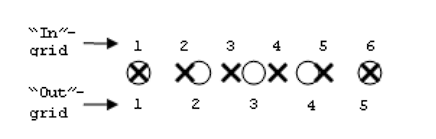
\includegraphics[width=100mm, keepaspectratio]{figures/poly_1d.png}
	\caption{A polyphase filter működése, 1 dimenzióban \cite{Xilinx_poly}} 
	\label{pic:poly_1d}
\end{figure}

Mint látjuk, a kimeneti pixel 4 féle fázisban lehet. Ezek a fázisok $0$, $1/4$, $2/4$, $3/4$. Ezeket úgy kaptuk meg hogy elosztottuk a kimeneti és bemeneti kép méretét (technikailag a kimenet-1 és a bemenet-1 méreteket), mellyel $5/4$ -et kaptunk, majd ezt mindig hozzáadtuk az előző pixel értékéhez, és így megkaptuk a kimeneti pixelek koordinátáit, a bemeneti képen: $0, 5/4, 10/4, 15/4, 20/4$, melyekből már látszanak az előbb megállapított fázisok. Ekkor tehát szűrő az alapján, hogy milyen fázisban van, más együtthatókat használ a környező pixelek súlyozására. Éppen ezért a polyphase szűrő nem együtthatókkal, hanem úgynevezett coefficient bank-al rendelkezik.

\subsection{Separable filter}

A polyphase szűrő egyszerűbb, és erőforrás takarékosabb megvalósításához érdemes a separable, vagyis úgynevezett szétválasztható szűrők fogalmának ismertetése. Ez csupán annyit takar, hogy pl a bilineáris szűrő megvalósításához hasonlóan, a szűrőnket szétdaraboljuk több, 1 dimenziós interpolációra. Ez a polyphase szűrőnél azt fogja jelenteni, hogyha pl 4-4 tap-es szűrőről van szó, akkor először a 4 oszlopon hajtunk végre egy interpolálást, amiből kapunk 4 értéket, majd végül ezen 4 értéken vízszíntes irányban hajtunk végre egy interpolálást, ezzel egyszerűsítve a filter architektúráját.\cite{Bart Wronski_2020} Ezt a mőködést a \ref{poly_2d} ábra szemlélteti.

\begin{figure}[!ht]
	\centering
	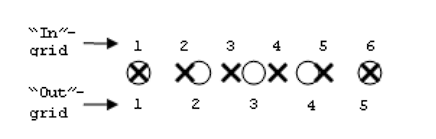
\includegraphics[width=100mm, keepaspectratio]{figures/poly_1d.png}
	\caption{Egy separable polyphase filter működése} 
	\label{pic:poly_2d}
\end{figure}

Fontos megjegyezni, hogy nem minden polyphase filter szétválasztható, ez csak akkor teljesül, ha olyan együtthatókat generálunk, amelyek erre képesek.


%----------------------------------------------------------------------------
\chapter{Bilineáris filter megvalósítása}
%----------------------------------------------------------------------------

Mivel ez volt az első félév ahol FPGA-val, és a verilog nyelvvel találkoztam, ezért első lépésnek azt tűztem ki célul, hogy megalkossam a bilineáris szűrőt. Ez elég sok trial and error-t tartalmazott, mert nem csak a digitális design, és a Vivado fejlesztői környezet, hanem a verilog nyelv is új volt számomra. 

Elsőnek egy olyan egyszerű modult alkottam meg, amelynek ha megadjuk a kimeneti és bemeneti kép méreteit, akkor képes meghatározni mindegyik kimeneti pixelnek a bemeneti képen a helyzetét. Ezután ezt a helyzetet outputként kiadja a modul, és a testbench visszaadja a 4 környező pixelt. 
Ezek után a 4 egymás melletti pixelből a modul előállítja a bilineáris filterhez szükséges súlyokat, majd végül elvégzi a megfelelő szorzásokat, és kiadja outputnak a kimeneti pixel értékét. 

Később ez a modul bővítve lett, hogy a bemenetre azt is meg lehessen adni, hogy hány csatornán érkeznek be a pixelek. Ha ez az érték 1, akkor szürkeárnyalatos képről beszélünk, és ha ez az érték 3, akkor színes, RGB képről beszélünk.
Ezen kívül egy állapotgépbe rendeztem a modult, hogy a későbbi fejezetben bemutatott sorbufferrel szinkronban tudjon működni a bilineáris filter.

\subsection{Számláló modul}

A Eddig sokat beszéltünk a backwards mappingról és különböző filter algoritmusokról, de arról nem, hogy hogyan is határozzuk meg a kimeneti kép pixeleit a bemeneti képen. Ezt a következő módon valósítottam meg. Raszter iránynak megfelelően, balról jobbra és fentről lefele, egyesével végigmentem a kimeneti kép pixelein. Ez egyszerűen megvalósítható, csak 2 számlálót kell inkrementálni, hogyha az x irányú számláló eléri a sornak a végét, akkor azt reseteljük, és inkrementáljuk az y irányú pixel számlálót. Ha az is eléri az kimeneti kép Y nagyságát, akkor készen vagyunk a képpel, ezeket resetelhetjük. 
Ezzel szinkronban, 2 másik számlálót is működtetünk, amely a mebemeti képen levő helyzetét számolja a kimeneti pixeleknek. Mindig amikor x irányban inkrementáljuk a kimeneti pixel számlálót, akkor az x irányú bemeneti pixel számlálót is inkrementáljuk a kimeneti és bemeneti képek arányaival. Mivel a pixelek számlálását 0 tól kezdjük, ezért ez az arányszám a következő lesz:

\begin{equation}
	scaleX=\frac{outputX-1}{inputX-1}, \quad és \quad scaleY=\frac{outputY-1}{inputY-1}
\end{equation}

Tehát a bemeneti és kimeneti képek méretének arányszáma az az érték, amivel inkrementálni kell a bemeneti kép pixel számlálóját. Ezt a működést a \ref{pic:bilinear_abra} ábra szemlélteti.

\begin{figure}[!ht]
	\centering
	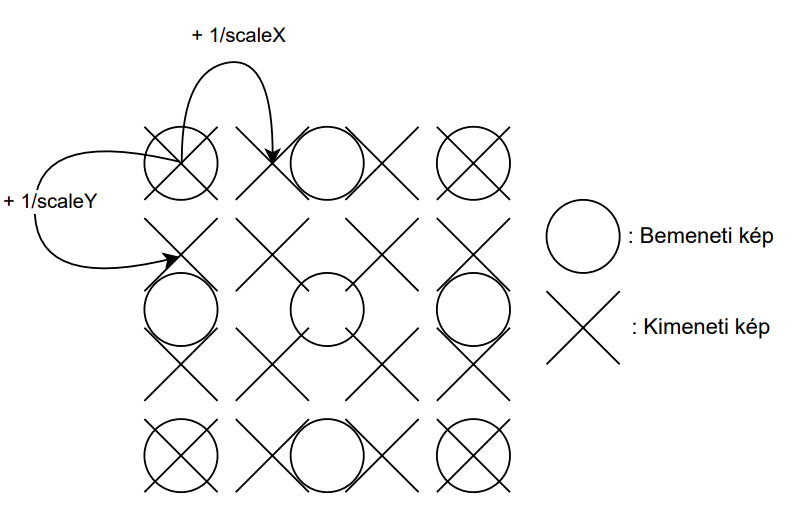
\includegraphics[width=100mm, keepaspectratio]{figures/bilinear_abra.png}
	\caption{A bilineáris filter számlálóinak működése} 
	\label{pic:bilinear_abra}
\end{figure}
\newpage
 Itt viszont észrevesszük, hogy ez az arány szám nem mindig egész szám. Éppen ezért ezt az arányszámot, és a bemeneti pixel számlálót is fix-pontos számként kell ábrázolnunk. Itt meg kellett ismerkednem a fix pontos számábrázolással, ami alapján sikerült is ezt a számláló egységet megvalósítanom. A számábrázolás során fontos volt, hogy a fix pontos számok maximum 18 biten legyenek ábrázolva, hiszen általában egy FPGA-ban ekkora bites számok szorzására képesek a LUT szorzók.

Fontos megjegyezni, hogy ezeket az arányszámokat inputként kell megadni, amelyeknek a legenerálására létrehoztam egy egyszerű python scriptet, melynek ha megadjuk a kimeneti kép és bemeneti kép méreteit, akkor az megadja a fix pontos ábrázolását a scale factoroknak.

A számláló egység tehát képes a kimeneti és bemeneti kép pixelein párhuzamosan végiszámolni. Ehhez készítettem egy szimulációt is, amelyen az látható, ahogy egy 512x512-es képet 800x800 ra méretezünk át. Ekkor ha a kimeneti kép közepén vagyunk, akkor a bemeneti kép közepén kell lenni, ami az \ref{pic:bilin_counter} ábrán levő szimuláción jól látszik hogy megtörténik.

\begin{figure}[!ht]
	\centering
	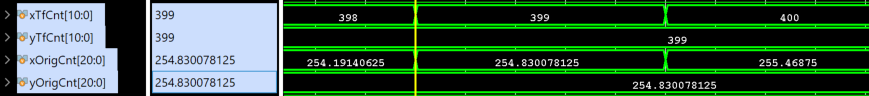
\includegraphics[width=100mm, keepaspectratio]{figures/bilin_counter.png}
	\caption{A bilineáris filter számlálóinak ellenőrzése} 
	\label{pic:bilin_counter}
\end{figure}

Ezután a bemeneti pixel számlálóknak a megfelelő formázása után (egész rész leválasztás) már be lehetett kérni a test bench-től a megfelelő 4 pixel értéket. Miután beérkeztek ezek a pixel értékek, kezdetét vehette a szorzó modul megvalósítása.

\subsection{Szorzó modul}

A szorzó modulban annak megfelelően, hogy hány csatornán érkeznek be a pixelek (1-szürkeárnyalatos, 3-RGB) egy generate blokk segítségével úgy van kiindexelve a bejövő pixel értékekből a megfelelő pixel értékek. Tehát ha 1 csatornáról van szó, akkor a bejövő pixel értékek csak 8 bitesek, de ha 3 csatornás a kép, akkor a bejövő pixelek 24 bitesek. Erre azért van szükség, mert kezdetben csak szürkeárnyalatos képen teszteltem a modult, és később valósítottam meg az RGB képek támogatását is. 

Itt csak megvalósításra kerültek a \ref{eq:mult} egyenletek szorásai. A kihívás itt viszont azt volt, hogy a szorzások megfelelő méretű regiszterekben legyenek tárolva, ne legyen túlcsordulás, ugyanis ha egy pl Q7.0 pixel értéket megszorzunk egy pl Q1.10 méretű együtthatóval, akkor egy Q8.10 méretű számot kapunk, amit csonkítani kell, és még tovább kell szorozni egy másik Q8.0 méretű számmal (felső és alsó interpoláció eredménye), majd végül a függőleges interpolációt is csonkítani kell. 
Ezeken kívül továbbá a megfelelő súlyokat kellő mennyiségő órajellel kellett késleltetni, hogy a felső és alsó interpoláció megfelelő súlyokkal dolgozzon, továbbá egy output data valid jelet is elő kellett állapítani, amit szintén megfelelő mennyiségű órajellel kellett késleltetni a beérkező data input valid jelhez képest.

Ezek után már működött a bilineáris szűrő, de annak érdekében hogy a később megvalósítandó sorbufferekkel szinkronban tudjon működni, egy állapotgépbe rendeztem a rendszer működését.

\subsection{Állapotgép}

A modulnak egy egyszerű állapotgépe van, mely a \ref{pic:bilin_state} ábrán látható.

\begin{figure}[!ht]
	\centering
	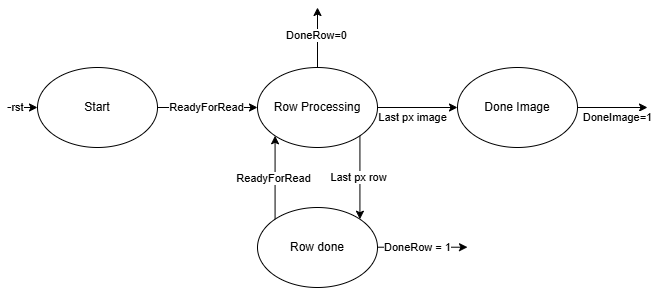
\includegraphics[width=120mm, keepaspectratio]{figures/bilin_state.png}
	\caption{A bilineáris filter állapotgépe} 
	\label{pic:bilin_state}
\end{figure}

A start állapotben inicializálunk minden változót, countert. Ezután, ha legalább 1 órajelig megkapjuk a readyForRead input jelet, akkor az azt jelenti, hogy a sorbuffer beolvasta a megfelelő sorokat, és készen áll az inputok kiadására. Tehát, ha a kimenetre kiírjuk egy pixelnek a koordinátáit (vagyis az oszlopának a sorszámát elég a sorbuffereknél), akkor az 1 órajel múlva meg fog jelenni a bemeneten. 

A processign állapotban egy soron végig halad a filter számlálója, és ezzel párhuzamosan a szorzó egység pár órajel késleltetéssel kiadja a megfelelő kimenő pixel értékét. Ha egy sor végére érünk, akkor a Row done állapotba megyünk át. Ha a kép végére értünk, (sor vége+ oszlopok vége) akkor a done image állapotba térünk.

A Row done állapotban egy soron végigértünk, a doeRow outputot magasra állítjuk, és várjuk hogya readyForRead input magas legyen. Amint ez magasra vált, a doneRow outputot alacsonyra állítjuk, és visszatérünk a Done image állapotba.

Az image Done állapotban a doneimage outputot magasra állítjuk, elkészült a kép. Innen resettel lehet a start állapotba juttatni a modult, és egy újabb kép feldolgozását megkezdeni.


% !TeX spellcheck = hu_HU
% !TeX encoding = UTF-8
% !TeX program = xelatex
%----------------------------------------------------------------------------
\chapter{A sorbuffer modul megvalósítása}
%----------------------------------------------------------------------------

Eddig úgy működtettem a test benchet a bilineáris filterhez, hogy a bemeneti képet (amit .raw fájlformátumban használtam, annak érdekében hogy pusztán csak a pixel adatokat tartalmazza, és egyéb header információkat ne) beolvastam egy tömbbe, és amikor a filter kért egy pixel értéket, azt csak szimplán kiindexeltem ebből a tömbből a kívánt sor és oszlop alapján. 
Ez a megoldás tesztelésre jó, de annak érdekében hogy a modul videó folyamot tudjon feldolgozni, ennél robosztusabb megoldásra van szükség. Éppen ezért megalkottam egy sorbuffer modult, aminek az a feladata, hogy eltárolja blokk-ram-okba azokat a sorokat amiket a filter éppen használ (a bilineáris filter esetén egyszerre csak 4 sort használ a szűrő, de polyphase esetén akár 4-et is használhat egyszerre), és ezekből a sorokból pedig már a megfelelő oszlopok pixeleit egyszerűen vissza lehet adni a filter számára.

Továbbá azért fontos még ez a sorbuffer modul, mert majd a továbbiakban, a bejövő video streamet és ezt a sorbuffer modult valamilyen axi interface-el fogom összekapcsolni, amivel a sorbuffer egyszerre tudja írni a blokk ramokat a bejövő video streamből, és közben a filterek számára a megfelelő pixelek értékeit pedig ki tudja adni.

\subsection{Blokkvázlat}

Tekintsük át a sorbuffer magas szintű működését először. Az architektúra blokkvázlata az \ref{pic:sorbuffer} ábrán látható. Mivel a bilineáris szűrő 2 bemeneti sor-t használ egyszerre, ezért ebben az esetben elegendő 4 sornyi blokkramot fenntartani a bufferben. 2 sornyi blokkramból párhuzamosan kiolvassuk a megfelelő oszlopok pixeleinek értékeit, és a maradék 2-be (vagy csak 1 be, vagy 0 ba, erről később) pedig beírjuk a filter által következőleg használt 2 sor értékeit. Tehát egy 2x-es kicsinyítés esetén, a kimeneti kép első sorához a bemeneti kép első két sorát olvassuk a blokkramokból, és közben a bemeneti kép következő 2 sor pixelértékeivel töltjük fel a másik 2 blokkramot, hiszen a kimeneti kép következő sorához, újabb 2 sorra van szükség.

\begin{figure}[!ht]
	\centering
	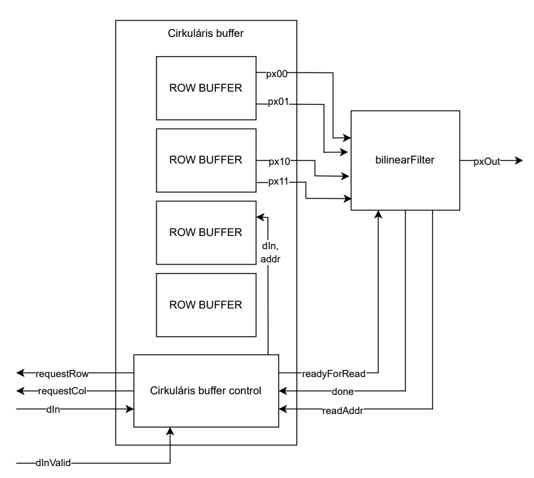
\includegraphics[width=120mm, keepaspectratio]{figures/sorbuffer.png}
	\caption{A sorbuffer architektúrája} 
	\label{pic:sorbuffer}
\end{figure}
\newpage

A működés egy cirkuláris bufferre épül, melyben $2^n$ db blokkram tud elhelyezkedni. Ha a filter $k$ sort használ használ fel a kimeneti pixel meghatározásához, akkor legalább $2k$ blokkramra van szükség a modulban annak érdekében, hogy a legrosszabb esetben is képes legyen a modul egyszerre írni a bejövő adatokat blokkramokba, és a filter tudja olvasni a számára szükséges adatokat. 

Tehát mivel a bilineáris filter 2 sort használ, ezért annál $n=2$, és mivel a polyphase filter pl 4 sort használhat, ezért ott $n=3$.

A cirkuláris bufferben van egy writePointer, és egy ReadPointer. Amikor egy újabb sort beolvasunk, akkor a writePointert inkrementáljuk, és egy újabb blokkramba olvassuk be a bemeneti adatokat. Amikor újabb sort akarunk koilvasni, akkor pedig a readPointert inkrementáljuk eggyel. Ha túlcsordulna bármelyik pointer, semmi probléma nincsen, a következő blokkram az akkor a 0. lesz akár olvasásról akár írásról van szó. Ezek a pointerek kezelik azt, hogy melyik blokkramból olvasunk ki és melyikbe írunk. Egyszerre csak egy blokkramba írunk, ugyanakkor mivel a bilineáris filternek 2 sorra van szükségea működésre, ezért egyszerre 2 sorból olvasunk. Ez nem probléma, hiszen abból a sorból sosem fogunk olvasni, amelyikbe éppen írunk, vagyis amelyikre éppen a writePointer mutat. Azonban ez az eset a kép legvégén megtörténhet, amikor is már nem olvasunk be több sort, és az utolsó sort olvassuk ki. Ekkor a write pointer és a read pointer ugyan arra a blokkramra mutat. Azonban ilyenkor tudjuk, hogy olvasni akarunk, ezért egy extra változó bevezetésével (forceRead) megoldhatjuk azt a problémát, hogy olvasás valósuljon meg a megadott címre, és ne pedig olvasás. 

Ezen kívül az olvasáskor mindig 2 sort kell olvasnunk, azt amelyikre a readpointer mutat, és a következőt. Ezeken felül az oszlopokból mindig azt kell olvasni amelyiket a bilineáris filter kér, (requestCol), és a következőt. Az alábbi kódrészlet azt mutatja be, hogy ez az írás olvasás logika hogyan van megvalósítva.

\begin{minted}{verilog}
wire [DATA_WIDTH-1:0] ramDataOutA [2**BUFFER_SIZE-1:0];
wire [DATA_WIDTH-1:0] ramDataOutB [2**BUFFER_SIZE-1:0];
//generating the RAM blocks 
generate
genvar i;
for(i = 0; i < 2**BUFFER_SIZE; i = i + 1)
begin : ram_generate
ram #(
.DATA_WIDTH(DATA_WIDTH),
.ADDRESS_WIDTH(ORIG_X_SIZE)
) ram_inst_i(
.clk( clk ),

//Port A is written to as well as read from. 
//When writing, this port cannot be read from.
.addrA( ((writeSelect == i) && !forceRead && writeEnable) ? requestCol : readAddress ),
.dataA( writeData ),													
.weA( ((writeSelect == i) && !forceRead) ? writeEnable : 1'b0 ),
.outA( ramDataOutA[i] ),

//portB is only read from, we are reading the next pixel 
.addrB( readAddress + 1'b1 ),
.dataB( writeData ),
.weB( 1'b0 ),
.outB( ramDataOutB[i] )
);
end
endgenerate

//Select which ram to read from
wire [BUFFER_SIZE-1:0]	readSelect0 = readSelect;
wire [BUFFER_SIZE-1:0]	readSelect1 = readSelect+1;

//Steer the output data to the right ports
assign readData00 = ramDataOutA[readSelect0];
assign readData01 = ramDataOutB[readSelect0];
assign readData10 = ramDataOutA[readSelect1];
assign readData11 = ramDataOutB[readSelect1];
\end{minted}

Mivel a ram egységek amiket példányosítottunk dual port ramok, ezért meg tudjuk csinálni hogy egyszerre 2 pixelt olvasunk ki belőlük. Éppen ezért a második porton csak olvasunk, és az első porton van lekezelve az írás logikája.

\subsection{Állapotgép}

A sorbuffer modulnak kicsit bonyolultabb állapotgépe van mint a bilinear filter modulnak. Az alapvető gondolat a működése mögött az az, hogy ebben a modulban is jelen van egy számláló, ami a bemeneti képen levő pixel helyzetét számolja (vagyis csak a sorának a helyzetét). Ha ennek a számlálónak az értéke nem billen át egy következő egész számra, (tehát pl 0-ról 0.6666-ra vált az értéke) akkor nem kell újabb sort beolvasnunk ahhoz, hogy a filter számára új adat elérhető legyen, hiszen ugyan azt a két sort fogja használni a következő kimeneti sor meghatározásához, mint amit eddig használt. 

Azonban ha a számláló értéke átbillen egy következő egészre (pl 0.666-ról 1.333-ra) akkor a filter következő kimeneti sorának az előállításához már a 0. bemeneti sorra nincs szükség, viszont a 2. bemeneti sorra igen. Ekkor beolvassuk az újabb bemeneti sort, és amikor végez a filter a jelenlegi sor feldolgozásával, a read pointert 1-el fogjuk növelni, ezáltal az outputra az 1. és 2. sor pixelei fognak majd kerülni olvasáskor.

Az utolsó eset, ha a sorszámláló értéke több mint 1 egésszel nőtt. Ekkor lényegtelen hogy mennyi egésszel nőtt az értéke, lehet az 2 is vagy akár 5, mindenképpen 2 új sort kell beolvasnunk, és a read pointert a következő sor feldolgozásánál 2 vel kell növelnünk, hogy a filter számára a 2 frissen beolvasott sor legyen elérhető.

Most, hogy megértettük a működés alapelvét, tekintsük meg az állapotgépet, és nézzük meg mi történik az egyes állapotokban.

\begin{figure}[!ht]
	\centering
	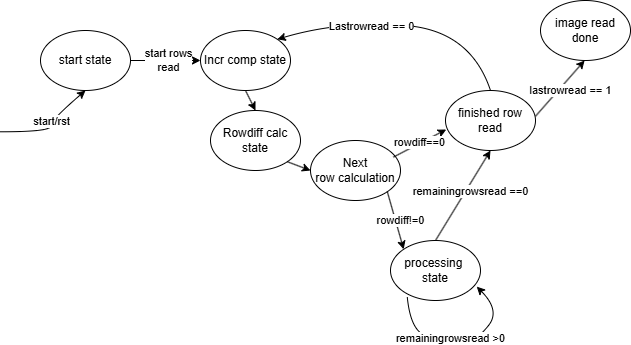
\includegraphics[width=120mm, keepaspectratio]{figures/sorbuffer_allapotgep.png}
	\caption{A sorbuffer állapotgépe} 
	\label{pic:sorbuffer_allapotgep}
\end{figure}

\begin{itemize}
	\item Start state: itt beolvasásra kerül az első 2 sor, hiszen azt mindenképpen be kell olvasni, ez lesz az első 2 sor amit a filter felhasznál. Amint ez befejeződött, a modul high-ra állítja a readyForRead outputot 1 órajelig, ezzel jelezve a filter modulnak hogy megkezdheti az első sor feldolgozását.
	\item Incr comp state: Kiszámoljuk a következő sornak az értékét, és az előzőnek az értékét elmentjük egy másik reg-be.
	\item Rowdiff calc state: Az incr comp state ben kiszámolt és elmentett két regiszter értékének a különbségét vesszük, és meghatározzuk, hogy mennyi egész szám került átlépésre a két sor között. Ezt az értéket a rowDiff regiszterbe mentjük.
	\item Next row calculation state: Itt az alapján hogy mi volt az előbb meghatározott rowdiff értéke, a következőket csinálhatjuk:
	\begin{itemize}
		\item rowDiff==0 esetén a következő sorok ugyan azok lesznek amik jelenleg is el vannak mentve, tehát nincs teendő, a finished row read state be ugrunk.
		\item rowDiff < NUMROWSTOSTORE mivel a bilineáris filter esetén 2 sort kell elmentenünk, ezért ha a rowDiff az ennél kevesebb (de 0 nál több, tehát 1), akkor a write pointert  eggyel növeljük, elmentjük hogy eggyel kevesebb sort kell beolvasnunk (bilineáris filter esetén ez 0 lesz), a remainingRowReads regiszterbe, és azt is elmentjük hogy mennyivel kell majd inkrementálni a read pointert, amikor a filter befejezte az előző sorok feldolgozását. Processing state-be ugrunk.
		\item a harmadik esetben 2 vel kell növelni (vagyis annyival amennyi sort eltárolunk a filter működéséhez) a write pointert, és azt is eltároljuk, hogy 2 vel kell megnövelni majd a read pointert. Ezen kívül azt is eltároljuk, hogy mennyi sor olvasása van még hátra (ez a bilineáris filter esetén 1 lesz). Processing state-be ugrunk.
	\end{itemize}
	\item Processing state: hasonlóan a start state hez, addig olvasunk be sorokat, ameddig be nem olvastuk a megfelelő mennyiségű sorokat, amit az előző state ben meghatároztunk. Ezek után a finished row state be ugrunk.
	\item finished row state: ha itt vagyunk, az azt jelenti hogy egy sort beolvastunk. Ez tehát azt jelenti, hogy a filter számára elérhetőek a következő sorok amiket használ, attól függetlenül, hogy azok ugyan azok-e vagy különbözőek attól, amiket most használ. Ebben a state ben ha a filter jelez hogy elkészült a sorok feldolgozásával, akkor újra visszaugrunk az incremenet compute state be, és előröl elkezdődik a folyamat, beolvassuk a filter számára szükséges következő sorokat. Ha azonban a kép végére értünk, akkor a finished image state be ugrunk, és a force read regisztert magasba rakjuk, hogy az utolsó sorból is ki tujda olvasni a filter a pixel értékeket.
	\item finished image state: készen vagyunk, beolvastuk az egész bemeneti képet. Resettel vagy start inputtal újra a start state be hozható az állapotgép
\end{itemize}

\subsection{Sorbuffer modul bővítése}

Ugyan a sorbuffer modult főként csak a bilineáris filterrel tudtam tesztelni, megpróbáltam egy olyan architektúrát létrehozni, amivel a polyphase filter esetén is használható lesz. Ugyan minden ilyen fejlesztést még nem sikerült implementálnom, de már gondolkodtam rajta hogy miket kellene változtatni. 
\begin{itemize}
	\item Nem lesz elég a filternek az oszlopot megadni hogy melyik pixeleet kéri a bemeneti képből, a sorok is kelleni fognak, hacsak nem bővítem a sorbuffer modul kimeneteit arra, hogy 4 sornak a pixeleit tudja egyszerre kiadni a kimenetre
	\item polyphase filternél nem azt kell majd itt számon tartani, hogy mi a kimeneti pixel bemeneti képén velő helye, hanem azt, hogy melyik sorban kezdődik a filter ablaka. Erre már előre létrehoztam egy numrowstostore parameter-t, aminek a segítségével ez számítható lesz.
\end{itemize}

\chapter{Eredmények, a projekt helyzete}

A projekt jelenlegi állása szerinte képes a bilineáris filterrel és a sorbufferekkel kiegészített modul segítségével tetszőlegesen átméretezni képeket. Mindkét modulhoz (sorbuffer modul, és bilineáris filter modul) készült testbench, amikkel azok működése ellenőrizhetővé vált. Ezen kívül elkészült egy harmadik testbench is, amiben a két modul integrálva van, és egymáshoz van csatlakoztatva. Néhány próba kép a \ref{sec:kepek} fejezetben található, ahol az eredeti 256x256 lena képet nagyítottam fel, majd egy tetszőleges méretűre méreteztem át.

A polyphase filter idő szűkében sajnos nem került még megvalósításra, még jelenleg fejlesztés alatt van, de mivel az irodalomkutatás része már megvan, ezért azta jövőben jóval egyszerűbb lesz megvalósítani, mint akár a félév elején az egyszerűbb bilineáris filtert. Ezt lehet az első továbbfejlesztésnek nevezni.

Ezen kívül a projekt jelenleg csak standalone képeket tud átméretezni, video folyamot nem, úgyhogy ezt a fejlesztést, hogy valamilyen axi interface-t csatlakoztatunk a sorbuffer modulhoz, és egy bemeneti video streamet juttatunk el annak, lehetne a második nagyobb fejlesztésnek is nevezni.

Harmadikként pedig a sorbuffer modul kisebb átdolgozsára szorul, hogy a polyphase filterrel is működni tudjon, de ezt már annak a fejezetében is említettem. A fejlesztés során próbáltam gondolni arra, hogy kicsit általánosabban működjön a sorbuffer modul, de mivel nem volt polyphase filter modulom elkészülve, amivel tesztelni tudtam volna, ezért ezt nem is tudtam 100\% ban így fejleszteni.

A projekt során rengeteget tanultam, mind a verilog nyelvből, mind FPGA működéséről, (hiszen ezekkel most találkoztam először) mind pedig általános képfeldolgozásról. Több külső eszközt kellett használnom hogy ellenőrizzem az eredményeim, ilyenek pl az IrfanView a .raw képek megtekintésére, vagy az ImHex hex editor, ahol a képeket pixel érték szinten tudtam vizsgálni. Ezen kívül segéd python scripteket is kellett írnom a modul teszteléséhez pl a scale factor megállapításához. A projekt forráskódja megtalálható a saját Githubomon, az alábbi linken: \url{https://github.com/NuunMoon/FPGA_scaler}


% Acknowledgements
%~~~~~~~~~~~~~~~~~~~~~~~~~~~~~~~~~~~~~~~~~~~~~~~~~~~~~~~~~~~~~~~~~~~~~~~~~~~~~~~~~~~~~~
%%----------------------------------------------------------------------------
\chapter*{\koszonetnyilvanitas}\addcontentsline{toc}{chapter}{\koszonetnyilvanitas}
%----------------------------------------------------------------------------

Ez nem kötelező, akár törölhető is. Ha a szerző szükségét érzi, itt lehet köszönetet nyilvánítani azoknak, akik hozzájárultak munkájukkal ahhoz, hogy a hallgató a szakdolgozatban vagy diplomamunkában leírt feladatokat sikeresen elvégezze. A konzulensnek való köszönetnyilvánítás sem kötelező, a konzulensnek hivatalosan is dolga, hogy a hallgatót konzultálja.


% List of Figures, Tables
%~~~~~~~~~~~~~~~~~~~~~~~~~~~~~~~~~~~~~~~~~~~~~~~~~~~~~~~~~~~~~~~~~~~~~~~~~~~~~~~~~~~~~~
%\listoffigures\addcontentsline{toc}{chapter}{\listfigurename}
%\listoftables\addcontentsline{toc}{chapter}{\listtablename}


% Bibliography
%~~~~~~~~~~~~~~~~~~~~~~~~~~~~~~~~~~~~~~~~~~~~~~~~~~~~~~~~~~~~~~~~~~~~~~~~~~~~~~~~~~~~~~
\addcontentsline{toc}{chapter}{\bibname}
\bibliography{bib/mybib}


% Appendix
%~~~~~~~~~~~~~~~~~~~~~~~~~~~~~~~~~~~~~~~~~~~~~~~~~~~~~~~~~~~~~~~~~~~~~~~~~~~~~~~~~~~~~~
%----------------------------------------------------------------------------
\appendix
%----------------------------------------------------------------------------
\chapter*{\fuggelek}\addcontentsline{toc}{chapter}{\fuggelek}
\setcounter{chapter}{\appendixnumber}
%\setcounter{equation}{0} % a fofejezet-szamlalo az angol ABC 6. betuje (F) lesz
\numberwithin{equation}{section}
\numberwithin{figure}{section}
\numberwithin{lstlisting}{section}
%\numberwithin{tabular}{section}

%----------------------------------------------------------------------------
\section{Próba képek}
\label{sec:kepek}
%----------------------------------------------------------------------------
\begin{figure}[!ht]
\centering
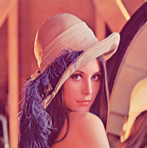
\includegraphics[width=150mm, keepaspectratio]{figures/lena_orig.png}
\caption{Lena eredeti változata, 256x256 méretű} 
\end{figure}

\begin{figure}[!ht]
	\centering
	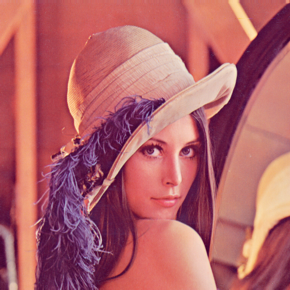
\includegraphics[width=150mm, keepaspectratio]{figures/lena_scaled.png}
	\caption{Lena 2x felnagyított változata, 512x512 méretű} 
\end{figure}

\begin{figure}[!ht]
	\centering
	
\includegraphics[width=150mm, keepaspectratio]{figures/lena_scaled_2.png}
	\caption{Lena tetszőlegesen nagyított változata, 800x150 méretű} 
\end{figure}
%----------------------------------------------------------------------------
%\clearpage\section{Válasz az ,,Élet, a világmindenség, meg minden'' kérdésére}
%----------------------------------------------------------------------------


%\label{page:last}
\end{document}
